\documentclass{article}
\usepackage{graphicx} % Required for inserting images
\usepackage{geometry}
\usepackage{titlesec}
\pagestyle{empty}

\titleformat{\section}[block]{\normalfont\Large\bfseries}{\thesection}{1em}{}
\titleformat{\subsection}[block]{\normalfont\Large}{\thesubsection}{2em}{} % Adds indentation
\begin{document}

\begin{center}
{\fontsize{36}{24}\selectfont \textbf{Peppermint}} \\
{\fontsize{18}{24}\selectfont \textit{Mentha x piperita}} \\
\vspace{30pt}
{\fontsize{20}{24}\selectfont Care instructions}\\
\vspace{30pt} 
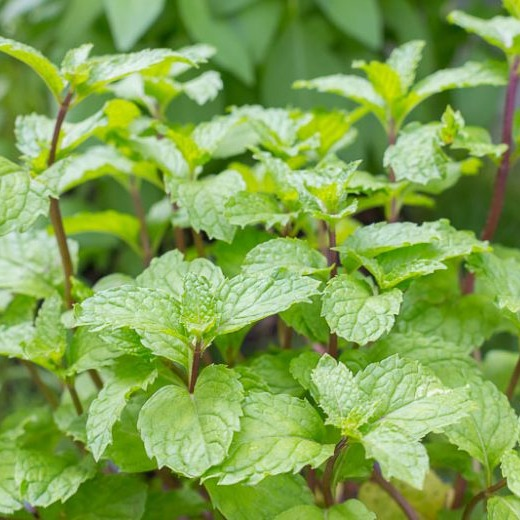
\includegraphics[width=1.0\textwidth]{intermediate/croppedimages/Peppermint.jpg}
\end{center}

\newgeometry{top=20mm, bottom=30mm, left=20mm, right=20mm}
\newpage

\section*{Info}
Peppermint (Mentha × piperita) is a fast-growing, aromatic herb that’s a natural hybrid of watermint and spearmint. Native to Europe and the Middle East, it thrives in temperate climates and is now cultivated globally. Peppermint spreads vigorously through underground rhizomes and is best grown in containers to control its growth. It prefers moist, rich, well-draining soil with a neutral to slightly acidic pH and grows best in full sun to partial shade. The plant is prized for its menthol-rich leaves, used in teas, culinary dishes, and natural remedies. Regular trimming encourages bushier growth and helps maintain its compact form.

\section*{Environmental Considerations}
\subsection*{Soil}
Moist, well-draining, slightly acidic soil with some organic matter
\subsection*{Upkeep}
Keep soil consistently moist; moderate to high humidity
\newline \newline \newline
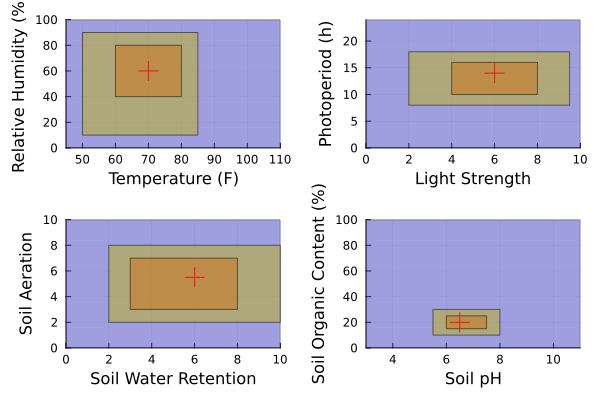
\includegraphics[width=.9\textwidth]{intermediate/plots/Peppermint.png}

\end{document}
